\sloppy
\documentclass[14pt,a4paper,oneside]{extarticle}	% Размер основного шрифта и формата листа
\usepackage{xltxtra}						% Используется для вывода логотипа XeLaTeX
\usepackage{xunicode}						% Кодировка документа
\usepackage{polyglossia}					% Загружает пакет многоязыковой верстки
\newfontfamily\russianfont{Book Antiqua}
%\setmainfont{Liberation Serif}						% Основной шрифт текста
\setmainfont{Book Antiqua}
\setdefaultlanguage{russian}				% Основной язык текста
\setotherlanguage{english}					% Дополнительный язык текста
\linespread{1}							% Межстрочный интервал выбран полуторным
\usepackage[left=2.5cm,
right=1.5cm,vmargin=2.5cm]{geometry} % Отступы по краям листа
\bibliographystyle{ugost2008}

\usepackage{xcolor}
\usepackage{hyperref}
% Цвета для гиперссылок
\definecolor{linkcolor}{HTML}{359B08} % цвет ссылок
\definecolor{urlcolor}{HTML}{799B03} % цвет гиперссылок
\hypersetup{pdfstartview=FitH,  linkcolor=linkcolor,urlcolor=urlcolor, colorlinks=true}

%---------------------------%
%---- Пакеты расширений ----%
%---------------------------%
\usepackage{xcolor}
\usepackage{hyperref}
% Цвета для гиперссылок
\definecolor{linkcolor}{HTML}{359B08} % цвет ссылок
\definecolor{urlcolor}{HTML}{799B03} % цвет гиперссылок
\hypersetup{pdfstartview=FitH,  linkcolor=linkcolor,urlcolor=urlcolor, colorlinks=true}


\usepackage{verbatim,indentfirst}
\usepackage{cite,enumerate,float}
\usepackage{amsmath,amssymb,amsthm,amsfonts}

%---------------------------%
%--- Вставка иллюстраций ---%
%---------------------------%
\usepackage{graphicx}
\usepackage{subfigure}
%\graphicspath{{Images/}}
\usepackage{fontspec}

\begin{document}
%	\pagestyle{empty} %  выключаенм нумерацию
	
%\setcounter{page}{3}% Нумерация начинается с третьей страницы
%\renewcommand{\contentsname}{\center{Содержание}}
%\tableofcontents
	
	\begin{center}
		%\addcontentsline{toc}{section}{Опыт 16. Нахождение центра масс}
		\subsection*{Прецессия гироскопа. Волчок}
	\end{center}
	
	\begin{figure}[H] 	
		\centering 	
		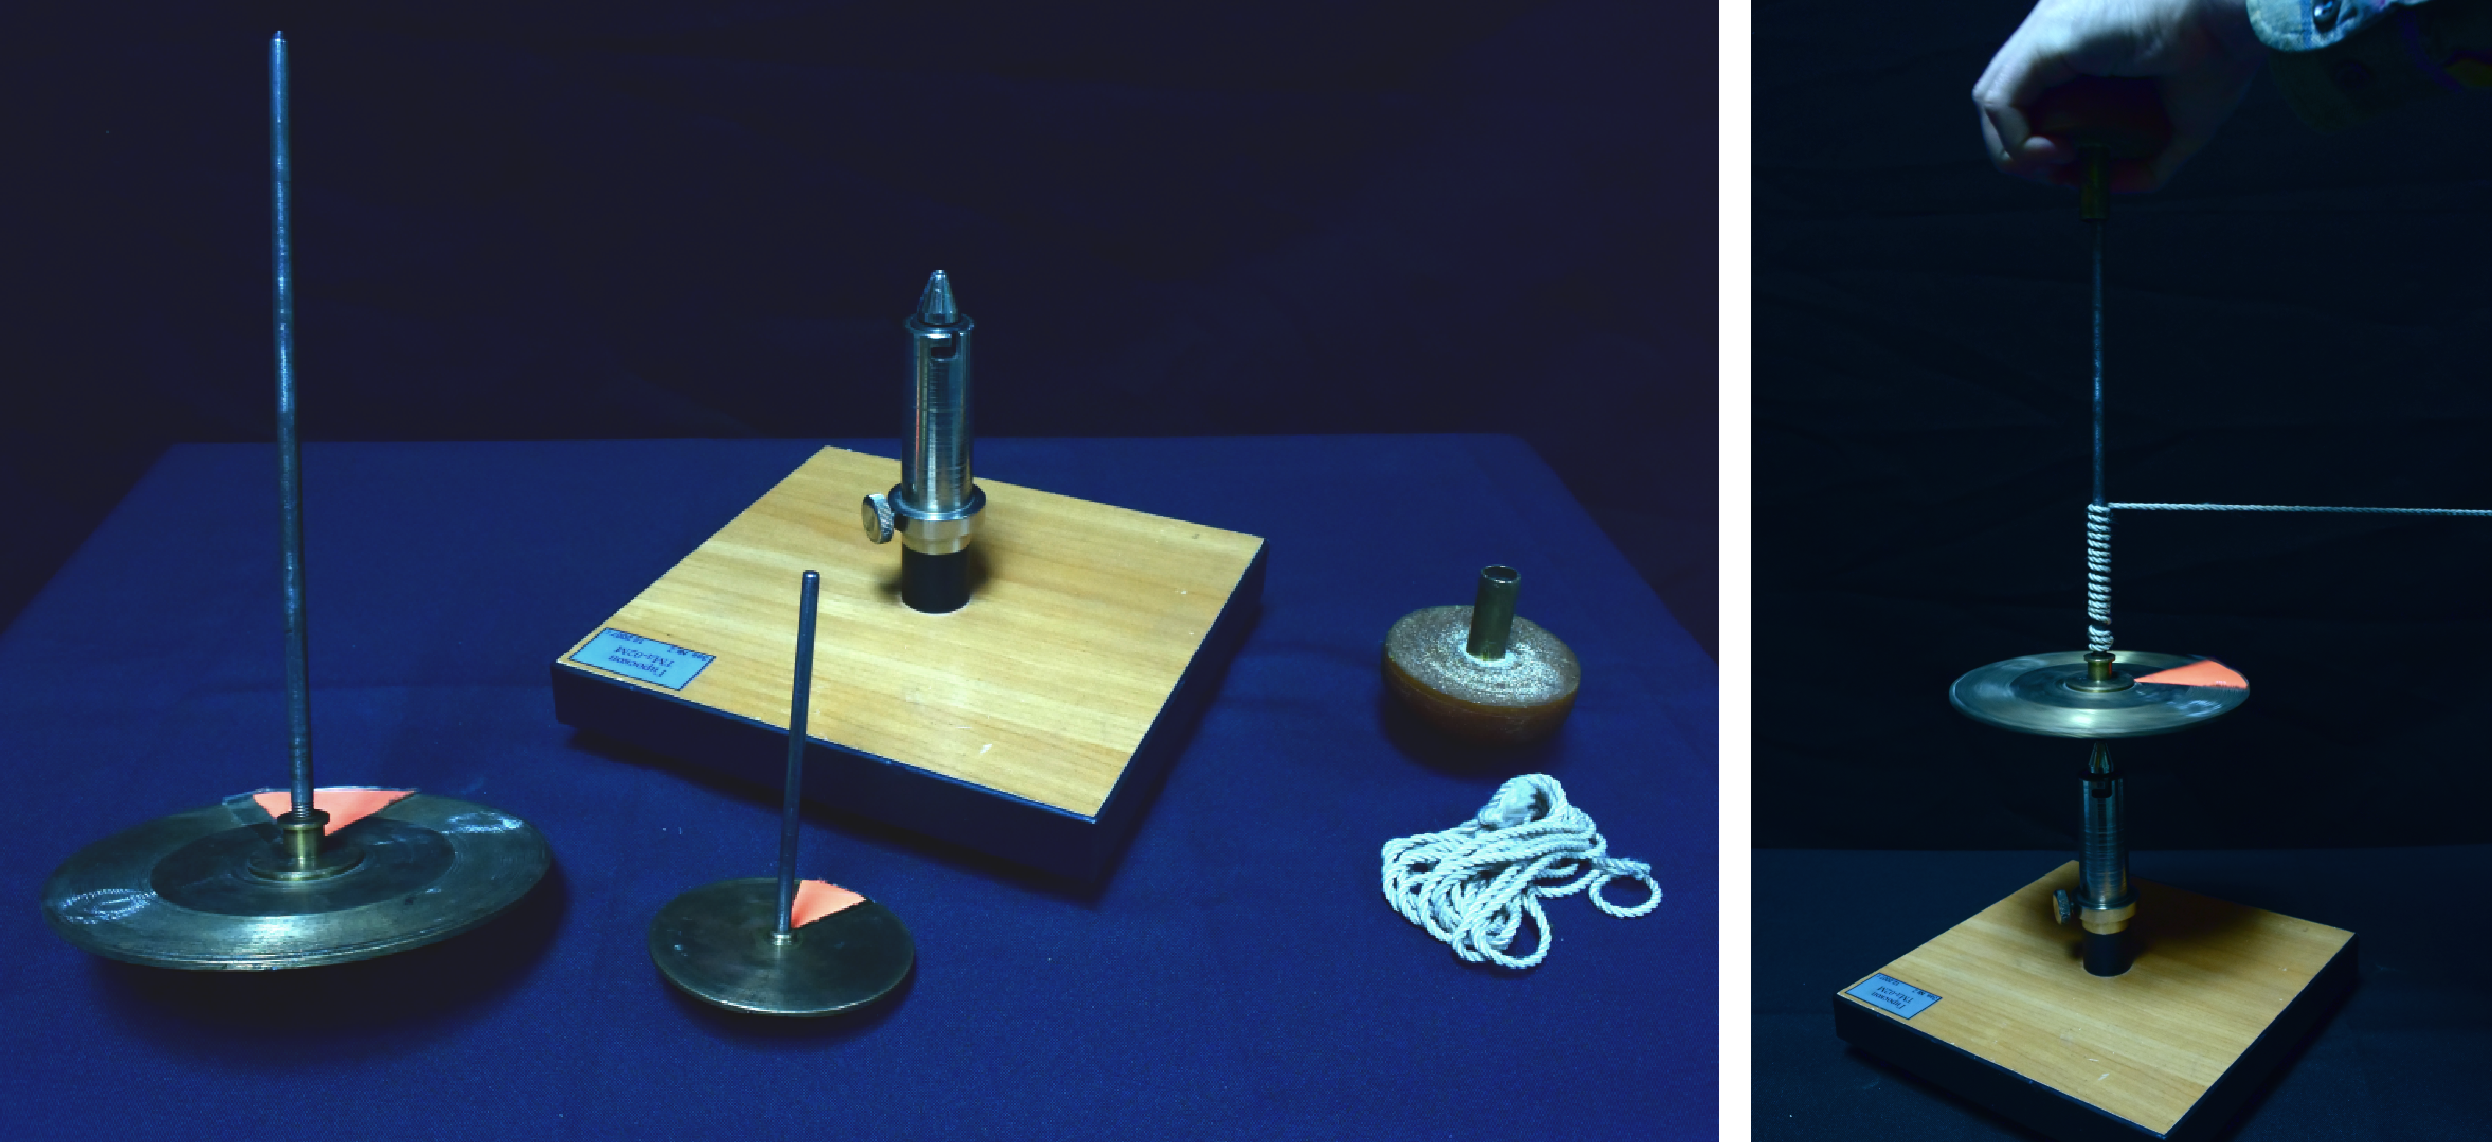
\includegraphics[width=0.9\linewidth]{gyro-4.png}
		\caption{Демонстрация гироскопического эффекта для различных волчков}
		\label{gyro-4}
	\end{figure}
	
	\subsection*{\underline{Оборудование:}}

			\begin{enumerate} 
			\item Два волчка различного размера и массы, волчок Томсона.
			\item Устройство для раскручивания волчка.
			\item Шнур или веревка.
		\end{enumerate}

\newpage
		\subsection*{\underline{Основные определения:}}
	
	Гироскоп — быстро вращающееся твердое тело, ось вращения которого может изменять 
	свое направление в пространстве.
	Гироскоп обладает рядом интересных свойств, наблюдаемых у вращающихся небесных тел, у артиллерийских снарядов, у детского волчка, у роторов турбин, установленных на судах, и др.
	
Свойства гироскопов проявляются при выполнении одного из условий, например, угловая скорость вращения гироскопа вокруг своей оси должна быть очень велика по сравнению с той угловой скоростью поворота оси в пространстве (другие свойства будут показаны в следующих демонстрациях).
	
Простейшим гироскопом является так называемый волчок, быстро вращающийся вокруг своей оси.  
Важно отметить, что если центр тяжести гироскопа совпадает с точкой опоры, то гироскоп называется астатическим (уравновешенным), 
в противном случае — тяжелым.

Прецессией волчка называется поворот самой оси вращения волчка под действием момента сил. В данной демонстрации момент силы тяжести вызывает прецессию волчка.

Если в какой-то момент времени действие силы прекратится, то одновременно прекратится прецессия и ось 
волчка мгновенно остановится, т. е. прецессионное движение гироскопа безынерционно.

Наряду с прецессиионным движением ось гироскопа при действии на нее силы может еще совершать так называемую нутацию — небольшие, 
но быстрые (обычно незаметные на глаз) колебания оси около ее среднего направления, быстро затухающимие из-за сопротивления воздуха.

Волчок Томсона, как правило, состоит из сферы со срезанной верхушкой. 
Это означает, что его центр тяжести находится ниже геометрического центра шара, из которого он изготовлен. 

\newpage
	\subsection*{\underline{Краткое описание:}}
	
	Демонстрация позволяет наблюдать за поведением волчка, опирающегося острием своей оси симметрии на неподвижную опору (рис.\ref{gyro-5},\textit{а}).
	Если попытаться поставить его в вертикальное положение, то он немедленно опрокинется, как только прекращается его поддержка. 
	Если центр тяжести расположен выше точки опоры, то малейшее смещение волчка в сторону от вертикального положения приводит к возникновению опрокидывающего момента силы тяжести.
	Вертикальное положение равновесия волчка является неустойчивым.
	Однако если волчку сообщить большую угловую скорость, то волчок будет располагаться вертикально, не падая, участвуя в прецессионном движении (рис.\ref{gyro-5},\textit{б}). 

У волчка роль центра подвеса играет точка опоры.
Со временем под действием сил трения угловая скорость вращения волчка начнет уменьшаться, при этом его ось отклоняется от вертикали на некоторый угол.
Под действием силы тяжести эта ось будет поворачиваться в направлении, перпендикулярном направлению силы тяжести, т.е. начнет прецессировать вокруг вертикальной оси (рис.\ref{gyro-5},\textit{в}).

			\begin{figure}[H] 	
	\centering 	
	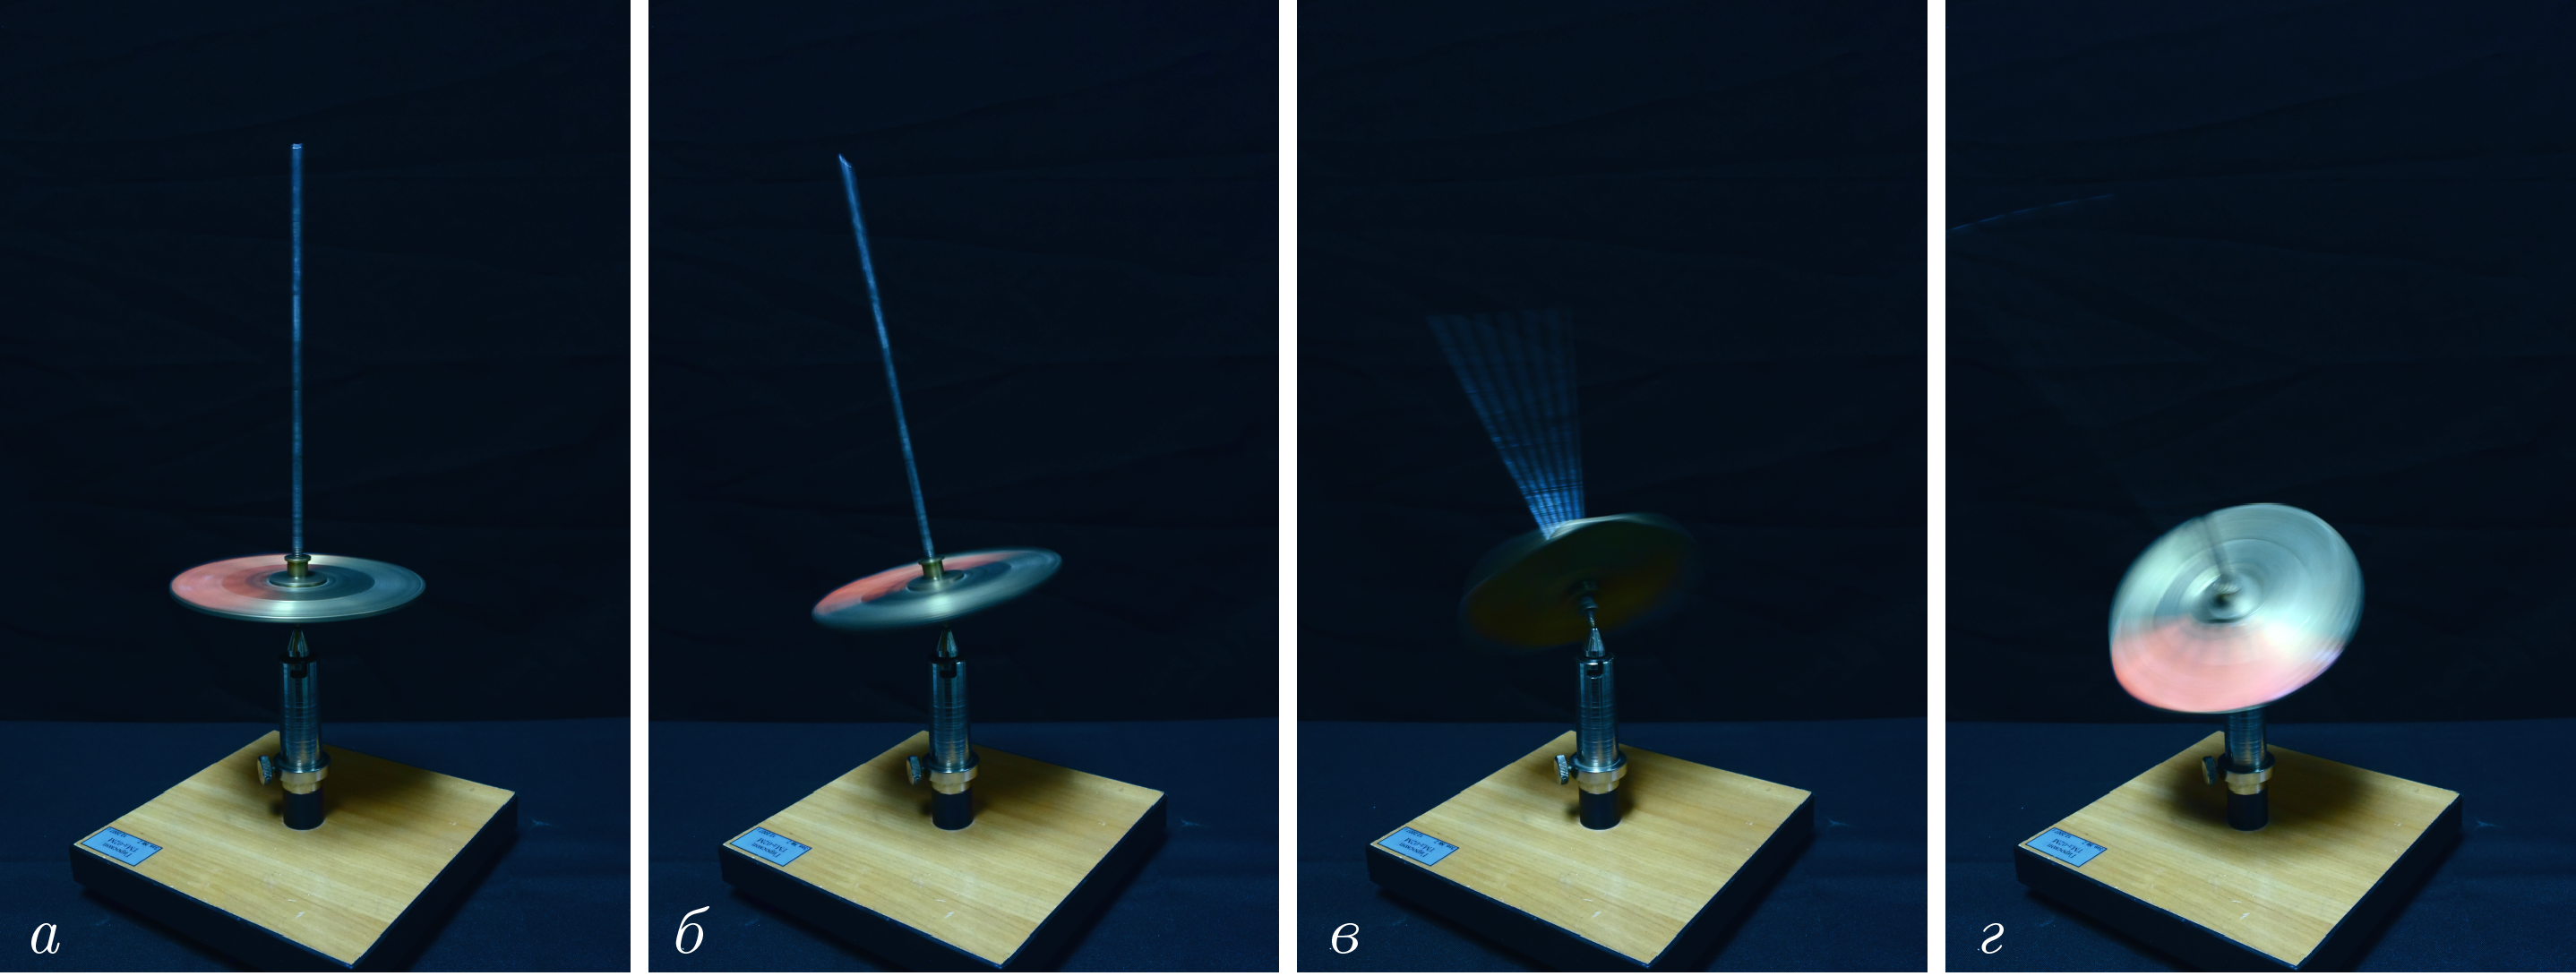
\includegraphics[width=0.9\linewidth]{gyro-5.png}
	\caption{Быстро вращающийся волчок не падает. Из-за трения угловая скорость собственного вращения уменьшается. По мере уменьшения скорости вращения, ось волчка спиралеобразно удаляется от вертикали, и волчок падает}
	\label{gyro-5}
\end{figure}

Чем меньше будет становится скорость вращения, тем заметнее будет прецессия волчка и тем больше станет угол отклонения оси волчка от вертикали.
Если скорость вращения станет очень малой, то волчок упадет.

\newpage
		\subsection*{\underline{Теория:}}
			
			\textit{Опыт 1}. Рассмотрим вращающийся дискообразный волчок.
			В начале когда угловая скорость велика, его ось практически вертикальна.
			Затем угловая скорость вращения под действием сил трения в точке  \textit{A} и о воздух уменьшается и волчок начинает прецессировать вокруг вертикальной оси, описывая коническую поверхность с вершиной в точке \textit{A} (рис.\ref{gyro-6},\textit{а}).
			
			\begin{figure}[H] 	
				\centering 	
				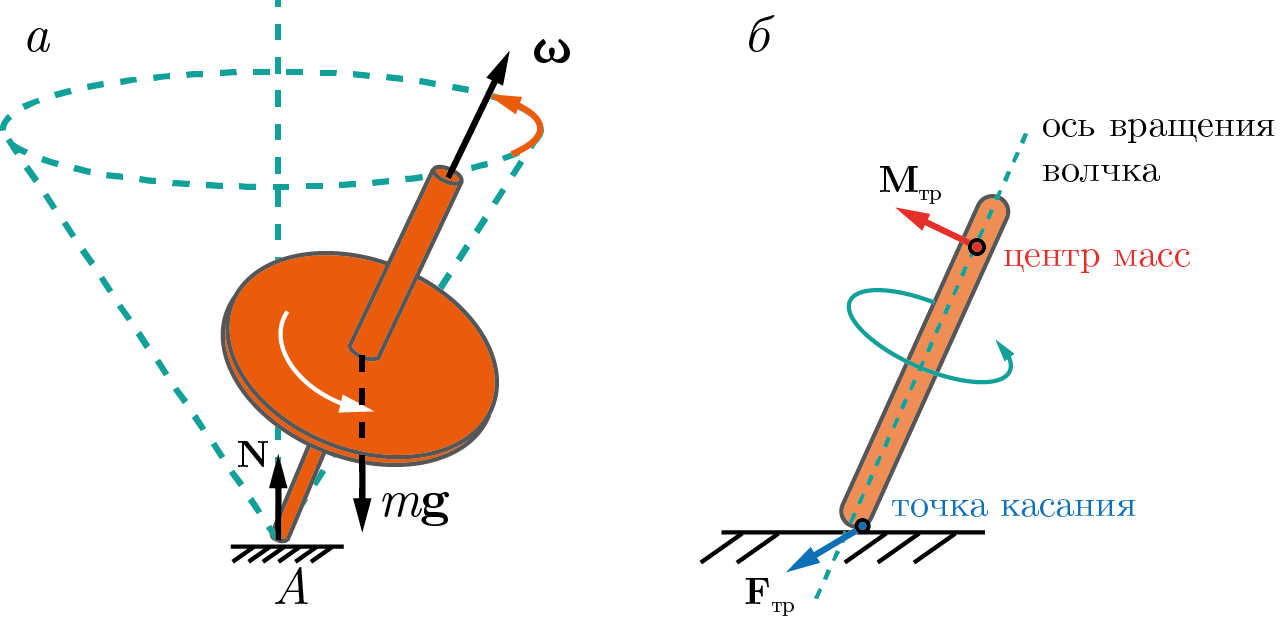
\includegraphics[width=0.75\linewidth]{gyro-6.png}
				\caption{Когда скорость вращения благодаря трению становится малой, ось волчка удаляется от вертикали, и волчок падает}
				\label{gyro-6}
			\end{figure}
			
			Рассмотрим силы действующие на волчок.
			Сила тяжести $ m\textbf{g} $ и сила реакции опоры $ \textbf{N} $ создают момент сил, стремящийся опрокинуть волчок. Это приводит к тому, что ось волчка смещается перпендикулярно плоскости действия этих сил, то есть прецессирует.
			Направление смещения оси показано на рис. красной стрелкой.
			
			Следует заметить, что прецессия оси волчка существовала и в самом начале его вращения из-за неизбежного толчка при раскручивании.
			
			Кроме момента пары сил  $ m\textbf{g} $ и $ \textbf{N} $  на волчок действует еще момент силы трения $ \textbf{F}_{\text{тр}} $ относительно центра масс волчка.
			На рис.\ref{gyro-6},\textit{б} показано увеличенное острие острие волчка. 
			Если точка касания острия с поверхностью не лежит на оси вращения волчка (волчок наклонился), то момент силы трения лежит в плоскости рисунка и направлен к вертикали. Изменение момента импульса волчка под действием момента силы трения тоже направлено к вертикальной оси; поэтому благодаря трению ось волчка стремится занять вертикальное положение. 	
			То есть, на наклонный волчок действуют два момента сил: момент пары сил — реакции опоры и силы тяжести, и момент силы трения. Движение волчка всегда происходит под действием этих двух моментов.
									
			\textit{Опыт 2}. При раскручивании волчка Томсона его ось непроизвольно отклоняется от вертикального положения.
			Однако из-за того, что волчок имеет сферическую форму, то точка его опоры в результате такого отклонения меняется.
			Ось же вращения волчка остается прежней — вертикальной, и не будет совпадать с его геометрической осью. 
			А так как центр тяжести волчка лежит ниже геометрического центра шарика, то в результате такого отклонения его центр тяжести уже не будет лежать на оси вращения (рис.\ref{gyro-7},\textit{а}).
			Он займет положение \textit{O'} и будет вращаться вместе с волчком около вертикальной оси.
			При вращении с большой угловой скоростью центр тяжести волчка будет подниматься точно так же, как поднимается шарик на нити, если нить раскручивать так, как показано на (рис.\ref{gyro-7},\textit{б}).	
				\begin{figure}[H] 	
					\centering 	
					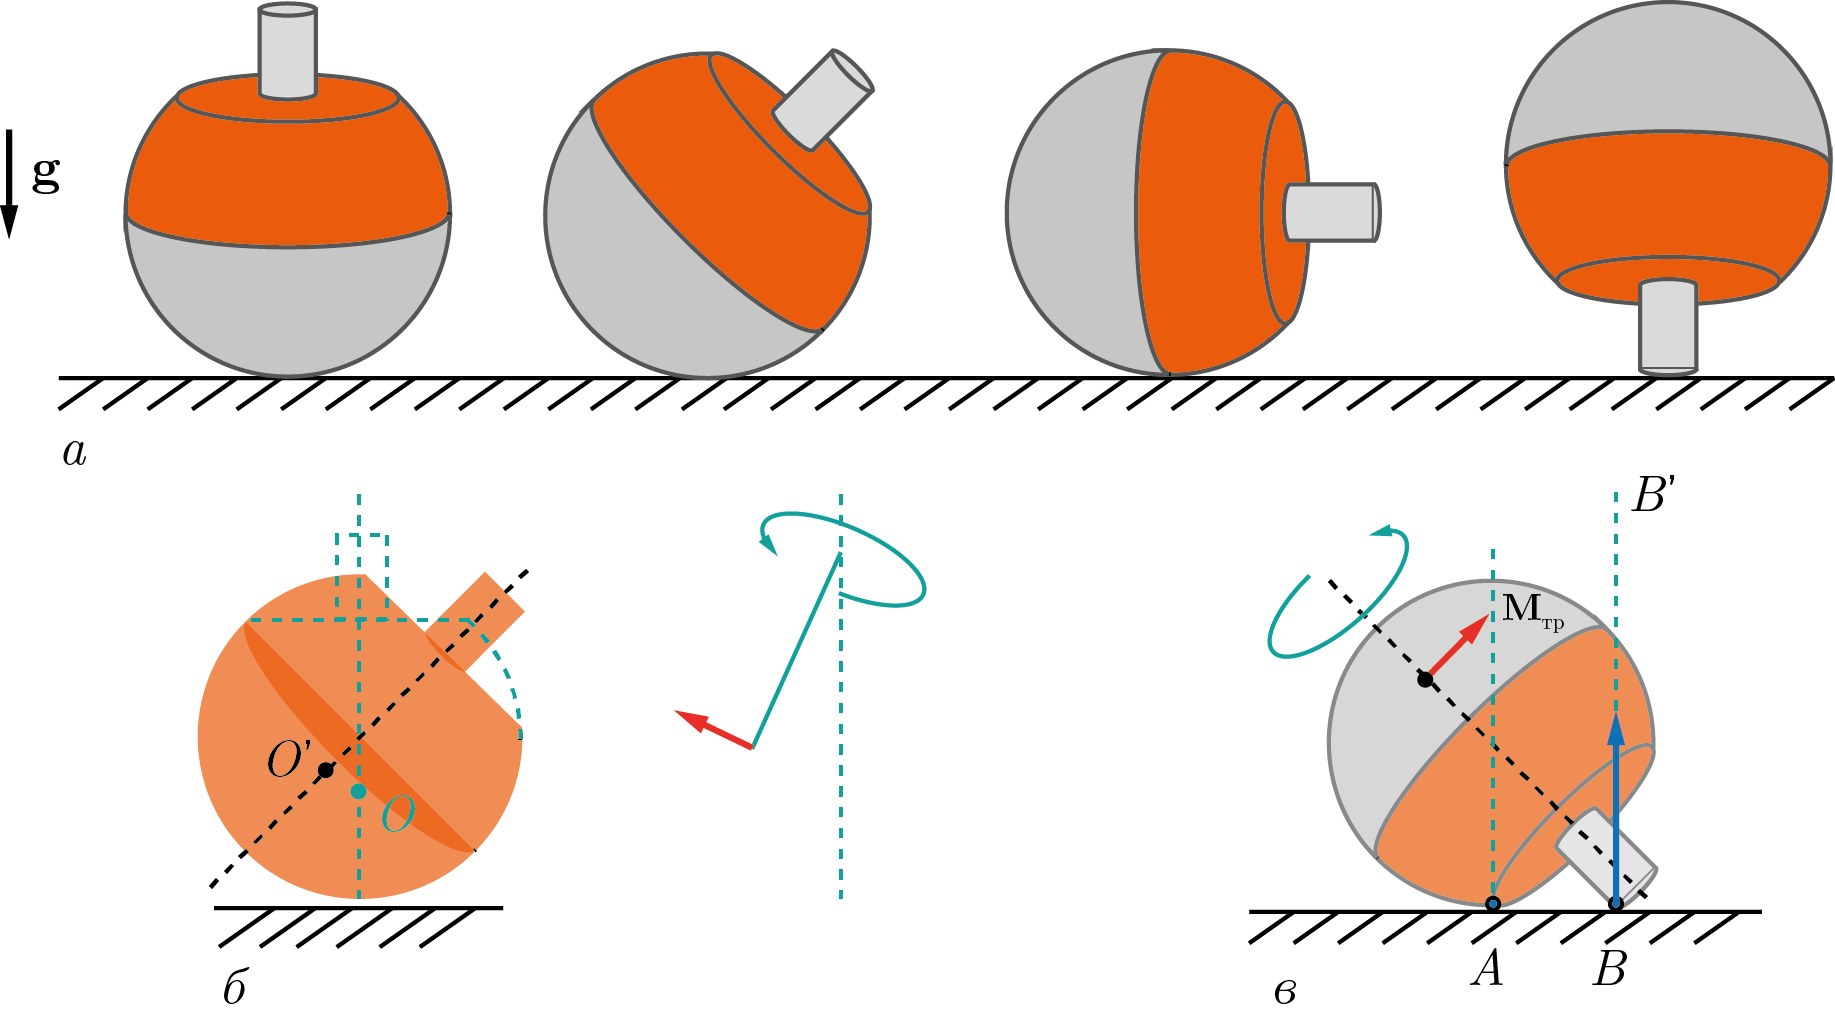
\includegraphics[width=0.9\linewidth]{gyro-7.png}
					\caption{Иллюстрация поведения вращающегося волчка Томсона, главной особенностью которого является подъем центра масса за счет момента силы трения}
					\label{gyro-7}
				\end{figure}	
					
			Волчок не задерживается в боковом положении, а по инерции проскакивает его, касаясь своей ножкой плоскости, на которой о вращается.
			Как только это произойдет, точка опоры волчка перескочит из точки  \textit{A} в точку  \textit{B} (рис.\ref{gyro-7},\textit{в}), и волчок вращаясь около своей оси, начнет прецессировать около оси \textit{BB'}. 
			Иными словами, волчок Томсона будет вести себя как «обыкновенный» волчок. 
			Под действием момента силы трения он совместит свою ось с вертикальной осью $ \text{ВВ}' $ и будет продолжать вращаться шариком кверху. 
			
			
%			быстро вращающийся вокруг своей оси ОА (рис. 1); 
%			ось ОА может изменять своё положение в пространстве, поскольку её конец А не закреплен. 
%			
%			Под действием силы Р (рис. 3) конец А оси АВ Г. будет отклонять не в сторону действия силы, как это было 
%			бы при невращающемся роторе, а в направлении, перпендикулярном к этой силе; в результате Г. вместе 
%			с рамкой 1 начнёт вращаться вокруг оси DE, притом не ускоренно, а с постоянной угловой скоростью. 
%			
%			Размахи этих колебаний у быстро вращающегося Г. очень малы и из-за неизбежного наличия сопротивлений быстро затухают. 
%			Это позволяет при решении большинства технических задач пренебречь нутацией и построить т. н. элементарную теорию 
%			Г., учитывающую только прецессию, скорость которой определяется формулой (1).
%			
%			У медленно вращающегося волчка нутационные колебания могут
%			быть довольно заметными и, слагаясь с прецессией, существенно изменить картину движения оси волчка: 
%			конец А оси будет описывать ясно видимую волнообразную или петлеобразную кривую, 
%			то отклоняясь от вертикали, то приближаясь к ней (рис. 5, б).
	
\end{document}
